\documentclass[twoside]{book}

% Packages required by doxygen
\usepackage{fixltx2e}
\usepackage{calc}
\usepackage{doxygen}
\usepackage[export]{adjustbox} % also loads graphicx
\usepackage{graphicx}
\usepackage[utf8]{inputenc}
\usepackage{makeidx}
\usepackage{multicol}
\usepackage{multirow}
\PassOptionsToPackage{warn}{textcomp}
\usepackage{textcomp}
\usepackage[nointegrals]{wasysym}
\usepackage[table]{xcolor}

% Font selection
\usepackage[T1]{fontenc}
\usepackage[scaled=.90]{helvet}
\usepackage{courier}
\usepackage{amssymb}
\usepackage{sectsty}
\renewcommand{\familydefault}{\sfdefault}
\allsectionsfont{%
  \fontseries{bc}\selectfont%
  \color{darkgray}%
}
\renewcommand{\DoxyLabelFont}{%
  \fontseries{bc}\selectfont%
  \color{darkgray}%
}
\newcommand{\+}{\discretionary{\mbox{\scriptsize$\hookleftarrow$}}{}{}}

% Page & text layout
\usepackage{geometry}
\geometry{%
  a4paper,%
  top=2.5cm,%
  bottom=2.5cm,%
  left=2.5cm,%
  right=2.5cm%
}
\tolerance=750
\hfuzz=15pt
\hbadness=750
\setlength{\emergencystretch}{15pt}
\setlength{\parindent}{0cm}
\setlength{\parskip}{3ex plus 2ex minus 2ex}
\makeatletter
\renewcommand{\paragraph}{%
  \@startsection{paragraph}{4}{0ex}{-1.0ex}{1.0ex}{%
    \normalfont\normalsize\bfseries\SS@parafont%
  }%
}
\renewcommand{\subparagraph}{%
  \@startsection{subparagraph}{5}{0ex}{-1.0ex}{1.0ex}{%
    \normalfont\normalsize\bfseries\SS@subparafont%
  }%
}
\makeatother

% Headers & footers
\usepackage{fancyhdr}
\pagestyle{fancyplain}
\fancyhead[LE]{\fancyplain{}{\bfseries\thepage}}
\fancyhead[CE]{\fancyplain{}{}}
\fancyhead[RE]{\fancyplain{}{\bfseries\leftmark}}
\fancyhead[LO]{\fancyplain{}{\bfseries\rightmark}}
\fancyhead[CO]{\fancyplain{}{}}
\fancyhead[RO]{\fancyplain{}{\bfseries\thepage}}
\fancyfoot[LE]{\fancyplain{}{}}
\fancyfoot[CE]{\fancyplain{}{}}
\fancyfoot[RE]{\fancyplain{}{\bfseries\scriptsize Generated by Doxygen }}
\fancyfoot[LO]{\fancyplain{}{\bfseries\scriptsize Generated by Doxygen }}
\fancyfoot[CO]{\fancyplain{}{}}
\fancyfoot[RO]{\fancyplain{}{}}
\renewcommand{\footrulewidth}{0.4pt}
\renewcommand{\chaptermark}[1]{%
  \markboth{#1}{}%
}
\renewcommand{\sectionmark}[1]{%
  \markright{\thesection\ #1}%
}

% Indices & bibliography
\usepackage{natbib}
\usepackage[titles]{tocloft}
\setcounter{tocdepth}{3}
\setcounter{secnumdepth}{5}
\makeindex

% Hyperlinks (required, but should be loaded last)
\usepackage{ifpdf}
\ifpdf
  \usepackage[pdftex,pagebackref=true]{hyperref}
\else
  \usepackage[ps2pdf,pagebackref=true]{hyperref}
\fi
\hypersetup{%
  colorlinks=true,%
  linkcolor=blue,%
  citecolor=blue,%
  unicode%
}

% Custom commands
\newcommand{\clearemptydoublepage}{%
  \newpage{\pagestyle{empty}\cleardoublepage}%
}

\usepackage{caption}
\captionsetup{labelsep=space,justification=centering,font={bf},singlelinecheck=off,skip=4pt,position=top}

%===== C O N T E N T S =====

\begin{document}

% Titlepage & ToC
\hypersetup{pageanchor=false,
             bookmarksnumbered=true,
             pdfencoding=unicode
            }
\pagenumbering{alph}
\begin{titlepage}
\vspace*{7cm}
\begin{center}%
{\Large Project\+\_\+\+Documentation }\\
\vspace*{1cm}
{\large Generated by Doxygen 1.8.13}\\
\end{center}
\end{titlepage}
\clearemptydoublepage
\pagenumbering{roman}
\tableofcontents
\clearemptydoublepage
\pagenumbering{arabic}
\hypersetup{pageanchor=true}

%--- Begin generated contents ---
\chapter{Namespace Index}
\section{Namespace List}
Here is a list of all namespaces with brief descriptions\+:\begin{DoxyCompactList}
\item\contentsline{section}{\hyperlink{namespacemain}{main} }{\pageref{namespacemain}}{}
\item\contentsline{section}{\hyperlink{namespacemain_1_1admin}{main.\+admin} }{\pageref{namespacemain_1_1admin}}{}
\item\contentsline{section}{\hyperlink{namespacemain_1_1apps}{main.\+apps} }{\pageref{namespacemain_1_1apps}}{}
\item\contentsline{section}{\hyperlink{namespacemain_1_1forms}{main.\+forms} }{\pageref{namespacemain_1_1forms}}{}
\item\contentsline{section}{\hyperlink{namespacemain_1_1models}{main.\+models} }{\pageref{namespacemain_1_1models}}{}
\item\contentsline{section}{\hyperlink{namespacemain_1_1tests}{main.\+tests} }{\pageref{namespacemain_1_1tests}}{}
\item\contentsline{section}{\hyperlink{namespacemain_1_1urls}{main.\+urls} }{\pageref{namespacemain_1_1urls}}{}
\item\contentsline{section}{\hyperlink{namespacemain_1_1views}{main.\+views} }{\pageref{namespacemain_1_1views}}{}
\end{DoxyCompactList}

\chapter{Hierarchical Index}
\section{Class Hierarchy}
This inheritance list is sorted roughly, but not completely, alphabetically\+:\begin{DoxyCompactList}
\item Model\begin{DoxyCompactList}
\item \contentsline{section}{main.\+models.\+dependent}{\pageref{classmain_1_1models_1_1dependent}}{}
\item \contentsline{section}{main.\+models.\+Leave}{\pageref{classmain_1_1models_1_1Leave}}{}
\item \contentsline{section}{main.\+models.\+Posts}{\pageref{classmain_1_1models_1_1Posts}}{}
\end{DoxyCompactList}
\item Model\+Form\begin{DoxyCompactList}
\item \contentsline{section}{main.\+forms.\+Leave\+Form}{\pageref{classmain_1_1forms_1_1LeaveForm}}{}
\item \contentsline{section}{main.\+forms.\+Posts\+Form}{\pageref{classmain_1_1forms_1_1PostsForm}}{}
\item \contentsline{section}{main.\+forms.\+select\+Form}{\pageref{classmain_1_1forms_1_1selectForm}}{}
\end{DoxyCompactList}
\item App\+Config\begin{DoxyCompactList}
\item \contentsline{section}{main.\+apps.\+Main\+Config}{\pageref{classmain_1_1apps_1_1MainConfig}}{}
\end{DoxyCompactList}
\end{DoxyCompactList}

\chapter{Class Index}
\section{Class List}
Here are the classes, structs, unions and interfaces with brief descriptions\+:\begin{DoxyCompactList}
\item\contentsline{section}{\hyperlink{classmain_1_1models_1_1dependent}{main.\+models.\+dependent} \\*Defines the model to store all the staff-\/supervisor mappings }{\pageref{classmain_1_1models_1_1dependent}}{}
\item\contentsline{section}{\hyperlink{classmain_1_1models_1_1Leave}{main.\+models.\+Leave} \\*Defines the model to store all the leave\+\_\+requests-\/related details }{\pageref{classmain_1_1models_1_1Leave}}{}
\item\contentsline{section}{\hyperlink{classmain_1_1forms_1_1LeaveForm}{main.\+forms.\+Leave\+Form} \\*Creates a form for the Leave model, using the django Model\+Form }{\pageref{classmain_1_1forms_1_1LeaveForm}}{}
\item\contentsline{section}{\hyperlink{classmain_1_1apps_1_1MainConfig}{main.\+apps.\+Main\+Config} }{\pageref{classmain_1_1apps_1_1MainConfig}}{}
\item\contentsline{section}{\hyperlink{classmain_1_1models_1_1Posts}{main.\+models.\+Posts} \\*Defines the model to store all the post-\/related details }{\pageref{classmain_1_1models_1_1Posts}}{}
\item\contentsline{section}{\hyperlink{classmain_1_1forms_1_1PostsForm}{main.\+forms.\+Posts\+Form} \\*Creates a form for the Posts model, using the django Model\+Form }{\pageref{classmain_1_1forms_1_1PostsForm}}{}
\item\contentsline{section}{\hyperlink{classmain_1_1forms_1_1selectForm}{main.\+forms.\+select\+Form} \\*Creates a form for the dependent model, using the django Model\+Form }{\pageref{classmain_1_1forms_1_1selectForm}}{}
\end{DoxyCompactList}

\chapter{File Index}
\section{File List}
Here is a list of all files with brief descriptions\+:\begin{DoxyCompactList}
\item\contentsline{section}{main/\hyperlink{____init_____8py}{\+\_\+\+\_\+init\+\_\+\+\_\+.\+py} }{\pageref{____init_____8py}}{}
\item\contentsline{section}{main/\hyperlink{admin_8py}{admin.\+py} }{\pageref{admin_8py}}{}
\item\contentsline{section}{main/\hyperlink{apps_8py}{apps.\+py} }{\pageref{apps_8py}}{}
\item\contentsline{section}{main/\hyperlink{forms_8py}{forms.\+py} }{\pageref{forms_8py}}{}
\item\contentsline{section}{main/\hyperlink{models_8py}{models.\+py} }{\pageref{models_8py}}{}
\item\contentsline{section}{main/\hyperlink{tests_8py}{tests.\+py} }{\pageref{tests_8py}}{}
\item\contentsline{section}{main/\hyperlink{urls_8py}{urls.\+py} }{\pageref{urls_8py}}{}
\item\contentsline{section}{main/\hyperlink{views_8py}{views.\+py} }{\pageref{views_8py}}{}
\end{DoxyCompactList}

\chapter{Namespace Documentation}
\hypertarget{namespacemain}{}\section{main Namespace Reference}
\label{namespacemain}\index{main@{main}}
\subsection*{Namespaces}
\begin{DoxyCompactItemize}
\item 
 \hyperlink{namespacemain_1_1admin}{admin}
\item 
 \hyperlink{namespacemain_1_1apps}{apps}
\item 
 \hyperlink{namespacemain_1_1forms}{forms}
\item 
 \hyperlink{namespacemain_1_1models}{models}
\item 
 \hyperlink{namespacemain_1_1tests}{tests}
\item 
 \hyperlink{namespacemain_1_1urls}{urls}
\item 
 \hyperlink{namespacemain_1_1views}{views}
\end{DoxyCompactItemize}

\hypertarget{namespacemain_1_1admin}{}\section{main.\+admin Namespace Reference}
\label{namespacemain_1_1admin}\index{main.\+admin@{main.\+admin}}

\hypertarget{namespacemain_1_1apps}{}\section{main.\+apps Namespace Reference}
\label{namespacemain_1_1apps}\index{main.\+apps@{main.\+apps}}
\subsection*{Classes}
\begin{DoxyCompactItemize}
\item 
class \hyperlink{classmain_1_1apps_1_1MainConfig}{Main\+Config}
\end{DoxyCompactItemize}

\hypertarget{namespacemain_1_1forms}{}\section{main.\+forms Namespace Reference}
\label{namespacemain_1_1forms}\index{main.\+forms@{main.\+forms}}
\subsection*{Classes}
\begin{DoxyCompactItemize}
\item 
class \hyperlink{classmain_1_1forms_1_1LeaveForm}{Leave\+Form}
\begin{DoxyCompactList}\small\item\em Creates a form for the Leave model, using the django Model\+Form. \end{DoxyCompactList}\item 
class \hyperlink{classmain_1_1forms_1_1PostsForm}{Posts\+Form}
\begin{DoxyCompactList}\small\item\em Creates a form for the Posts model, using the django Model\+Form. \end{DoxyCompactList}\item 
class \hyperlink{classmain_1_1forms_1_1selectForm}{select\+Form}
\begin{DoxyCompactList}\small\item\em Creates a form for the dependent model, using the django Model\+Form. \end{DoxyCompactList}\end{DoxyCompactItemize}

\hypertarget{namespacemain_1_1models}{}\section{main.\+models Namespace Reference}
\label{namespacemain_1_1models}\index{main.\+models@{main.\+models}}
\subsection*{Classes}
\begin{DoxyCompactItemize}
\item 
class \hyperlink{classmain_1_1models_1_1dependent}{dependent}
\begin{DoxyCompactList}\small\item\em Defines the model to store all the staff-\/supervisor mappings. \end{DoxyCompactList}\item 
class \hyperlink{classmain_1_1models_1_1Leave}{Leave}
\begin{DoxyCompactList}\small\item\em Defines the model to store all the leave\+\_\+requests-\/related details. \end{DoxyCompactList}\item 
class \hyperlink{classmain_1_1models_1_1Posts}{Posts}
\begin{DoxyCompactList}\small\item\em Defines the model to store all the post-\/related details. \end{DoxyCompactList}\end{DoxyCompactItemize}

\hypertarget{namespacemain_1_1tests}{}\section{main.\+tests Namespace Reference}
\label{namespacemain_1_1tests}\index{main.\+tests@{main.\+tests}}

\hypertarget{namespacemain_1_1urls}{}\section{main.\+urls Namespace Reference}
\label{namespacemain_1_1urls}\index{main.\+urls@{main.\+urls}}
\subsection*{Variables}
\begin{DoxyCompactItemize}
\item 
string \hyperlink{namespacemain_1_1urls_a51dcca3e024577b219fd64d918455026}{app\+\_\+name} = \char`\"{}main\char`\"{}
\item 
list \hyperlink{namespacemain_1_1urls_a49ff062cbecb056ec955c38ee8b784c3}{urlpatterns}
\begin{DoxyCompactList}\small\item\em contain the url patterns and their respective views \end{DoxyCompactList}\end{DoxyCompactItemize}


\subsection{Detailed Description}
\begin{DoxyVerb}Used to perform certain views against certain url requests
Is a mapping between URL path expressions to Python functions (the views).
\end{DoxyVerb}
 

\subsection{Variable Documentation}
\mbox{\Hypertarget{namespacemain_1_1urls_a51dcca3e024577b219fd64d918455026}\label{namespacemain_1_1urls_a51dcca3e024577b219fd64d918455026}} 
\index{main\+::urls@{main\+::urls}!app\+\_\+name@{app\+\_\+name}}
\index{app\+\_\+name@{app\+\_\+name}!main\+::urls@{main\+::urls}}
\subsubsection{\texorpdfstring{app\+\_\+name}{app\_name}}
{\footnotesize\ttfamily string main.\+urls.\+app\+\_\+name = \char`\"{}main\char`\"{}}

\mbox{\Hypertarget{namespacemain_1_1urls_a49ff062cbecb056ec955c38ee8b784c3}\label{namespacemain_1_1urls_a49ff062cbecb056ec955c38ee8b784c3}} 
\index{main\+::urls@{main\+::urls}!urlpatterns@{urlpatterns}}
\index{urlpatterns@{urlpatterns}!main\+::urls@{main\+::urls}}
\subsubsection{\texorpdfstring{urlpatterns}{urlpatterns}}
{\footnotesize\ttfamily list main.\+urls.\+urlpatterns}

{\bfseries Initial value\+:}
\begin{DoxyCode}
1 =  [
2     path(\textcolor{stringliteral}{''}, views.homepage, name=\textcolor{stringliteral}{"homepage"}),
3     path(\textcolor{stringliteral}{'posts/'}, views.posts, name=\textcolor{stringliteral}{"posts"}),
4     path(\textcolor{stringliteral}{'register/'},views.register, name=\textcolor{stringliteral}{"register"}),
5     path(\textcolor{stringliteral}{'staff/'},views.register\_staff, name=\textcolor{stringliteral}{"register\_staff"}),
6     path(\textcolor{stringliteral}{'supervisor/'},views.register\_supervisor, name=\textcolor{stringliteral}{"register\_supervisor"}),
7     path(\textcolor{stringliteral}{"logout/"}, views.logout\_request, name=\textcolor{stringliteral}{"logout"}),
8     path(\textcolor{stringliteral}{"login/"}, views.login\_request, name=\textcolor{stringliteral}{"login"}),
9     path(\textcolor{stringliteral}{"add\_post/"}, views.create\_posts, name=\textcolor{stringliteral}{"create\_post"}),
10     path(\textcolor{stringliteral}{"apply\_leave/"}, views.leave, name=\textcolor{stringliteral}{"apply\_leave"}),
11     path(\textcolor{stringliteral}{"leave\_requests/"},views.leave\_requests, name=\textcolor{stringliteral}{'leave\_requests'}),
12     path(\textcolor{stringliteral}{"select\_supervisor/"}, views.select\_supervisor, name=\textcolor{stringliteral}{'select\_supervisor'}),
13 ]
\end{DoxyCode}


contain the url patterns and their respective views 


\hypertarget{namespacemain_1_1views}{}\section{main.\+views Namespace Reference}
\label{namespacemain_1_1views}\index{main.\+views@{main.\+views}}
\subsection*{Functions}
\begin{DoxyCompactItemize}
\item 
def \hyperlink{namespacemain_1_1views_a65a9dba6e3878ee1da013593b60345d4}{homepage} (request)
\begin{DoxyCompactList}\small\item\em Defines what action to perform when the view \textquotesingle{}homepage\textquotesingle{} is called from urls. \end{DoxyCompactList}\item 
def \hyperlink{namespacemain_1_1views_a33ddb0f904d196b5830dbb9a1a8f1282}{posts} (request)
\begin{DoxyCompactList}\small\item\em Defines what action to perform when the view \textquotesingle{}posts\textquotesingle{} is called from urls. \end{DoxyCompactList}\item 
def \hyperlink{namespacemain_1_1views_acdd49ab16815f9d6cb3e88feab0bfa80}{leave\+\_\+requests} (request)
\begin{DoxyCompactList}\small\item\em Defines what action to perform when the view \textquotesingle{}leave\+\_\+requests\textquotesingle{} is called from urls. \end{DoxyCompactList}\item 
def \hyperlink{namespacemain_1_1views_abdf62da100e2d6945871318f111c478c}{select\+\_\+supervisor} (request)
\begin{DoxyCompactList}\small\item\em Defines what action to perform when the view \textquotesingle{}select\+\_\+supervisor\textquotesingle{} is called from urls. \end{DoxyCompactList}\item 
def \hyperlink{namespacemain_1_1views_a5188f01b8c7ed850b1f946afb34d183a}{create\+\_\+posts} (request)
\begin{DoxyCompactList}\small\item\em Defines what action to perform when the view \textquotesingle{}create\+\_\+posts\textquotesingle{} is called from urls. \end{DoxyCompactList}\item 
def \hyperlink{namespacemain_1_1views_a0e05992f5c64ffb3cd35ddc581399e31}{leave} (request)
\begin{DoxyCompactList}\small\item\em Defines what action to perform when the view \textquotesingle{}leave\textquotesingle{} is called from urls. \end{DoxyCompactList}\item 
def \hyperlink{namespacemain_1_1views_a36b45d6ab9335da129aeab31c613726a}{register} (request)
\begin{DoxyCompactList}\small\item\em Defines what action to perform when the view \textquotesingle{}register\textquotesingle{} is called from urls. \end{DoxyCompactList}\item 
def \hyperlink{namespacemain_1_1views_afa83b35a6a0c354a6d9878bc3584aae4}{register\+\_\+staff} (request)
\begin{DoxyCompactList}\small\item\em Defines what action to perform when the view \textquotesingle{}register\+\_\+staff\textquotesingle{} is called from urls. \end{DoxyCompactList}\item 
def \hyperlink{namespacemain_1_1views_a26d1574cf1c0681b1589baf8f2840e4a}{register\+\_\+supervisor} (request)
\begin{DoxyCompactList}\small\item\em Defines what action to perform when the view \textquotesingle{}register\+\_\+supervisor\textquotesingle{} is called from urls. \end{DoxyCompactList}\item 
def \hyperlink{namespacemain_1_1views_a19ef1e1ff8dc4a8b7f24c011a69c56f5}{logout\+\_\+request} (request)
\begin{DoxyCompactList}\small\item\em Defines what action to perform when the view \textquotesingle{}logout\+\_\+request\textquotesingle{} is called from urls. \end{DoxyCompactList}\item 
def \hyperlink{namespacemain_1_1views_aa4b0b085bb5782a107fce5e03228e97b}{login\+\_\+request} (request)
\begin{DoxyCompactList}\small\item\em Defines what action to perform when the view \textquotesingle{}login\+\_\+request\textquotesingle{} is called from urls. \end{DoxyCompactList}\end{DoxyCompactItemize}


\subsection{Function Documentation}
\mbox{\Hypertarget{namespacemain_1_1views_a5188f01b8c7ed850b1f946afb34d183a}\label{namespacemain_1_1views_a5188f01b8c7ed850b1f946afb34d183a}} 
\index{main\+::views@{main\+::views}!create\+\_\+posts@{create\+\_\+posts}}
\index{create\+\_\+posts@{create\+\_\+posts}!main\+::views@{main\+::views}}
\subsubsection{\texorpdfstring{create\+\_\+posts()}{create\_posts()}}
{\footnotesize\ttfamily def main.\+views.\+create\+\_\+posts (\begin{DoxyParamCaption}\item[{}]{request }\end{DoxyParamCaption})}



Defines what action to perform when the view \textquotesingle{}create\+\_\+posts\textquotesingle{} is called from urls. 

Used to create new posts for job by the supervisors, for the staffs. Sends the template create\+\_\+post.\+html as H\+T\+T\+P\+Response, along with the django form for getting the post details posted by the current user, as the template’s context for rendering. 
\begin{DoxyParams}{Parameters}
{\em request} & The H\+T\+T\+P\+Request object \\
\hline
\end{DoxyParams}
\begin{DoxyReturn}{Returns}
H\+T\+T\+P\+Response object containing the template and context containing the django form Posts\+Form 
\end{DoxyReturn}
\mbox{\Hypertarget{namespacemain_1_1views_a65a9dba6e3878ee1da013593b60345d4}\label{namespacemain_1_1views_a65a9dba6e3878ee1da013593b60345d4}} 
\index{main\+::views@{main\+::views}!homepage@{homepage}}
\index{homepage@{homepage}!main\+::views@{main\+::views}}
\subsubsection{\texorpdfstring{homepage()}{homepage()}}
{\footnotesize\ttfamily def main.\+views.\+homepage (\begin{DoxyParamCaption}\item[{}]{request }\end{DoxyParamCaption})}



Defines what action to perform when the view \textquotesingle{}homepage\textquotesingle{} is called from urls. 

Sends the template index.\+html as H\+T\+T\+P\+Response (for the homepage)


\begin{DoxyParams}{Parameters}
{\em request} & The H\+T\+T\+P\+Request object \\
\hline
\end{DoxyParams}
\begin{DoxyReturn}{Returns}
H\+T\+T\+P\+Response object conatining the template for homepage 
\end{DoxyReturn}
\mbox{\Hypertarget{namespacemain_1_1views_a0e05992f5c64ffb3cd35ddc581399e31}\label{namespacemain_1_1views_a0e05992f5c64ffb3cd35ddc581399e31}} 
\index{main\+::views@{main\+::views}!leave@{leave}}
\index{leave@{leave}!main\+::views@{main\+::views}}
\subsubsection{\texorpdfstring{leave()}{leave()}}
{\footnotesize\ttfamily def main.\+views.\+leave (\begin{DoxyParamCaption}\item[{}]{request }\end{DoxyParamCaption})}



Defines what action to perform when the view \textquotesingle{}leave\textquotesingle{} is called from urls. 

Used to create new leave requests by the staffs. Sends the template apply\+\_\+leave.\+html as H\+T\+T\+P\+Response, along with the django form for getting the leave request details posted by the current user, as the template’s context for rendering. 
\begin{DoxyParams}{Parameters}
{\em request} & The H\+T\+T\+P\+Request object \\
\hline
\end{DoxyParams}
\begin{DoxyReturn}{Returns}
H\+T\+T\+P\+Response object containing the template and context containing the django form Leave\+Form 
\end{DoxyReturn}
\mbox{\Hypertarget{namespacemain_1_1views_acdd49ab16815f9d6cb3e88feab0bfa80}\label{namespacemain_1_1views_acdd49ab16815f9d6cb3e88feab0bfa80}} 
\index{main\+::views@{main\+::views}!leave\+\_\+requests@{leave\+\_\+requests}}
\index{leave\+\_\+requests@{leave\+\_\+requests}!main\+::views@{main\+::views}}
\subsubsection{\texorpdfstring{leave\+\_\+requests()}{leave\_requests()}}
{\footnotesize\ttfamily def main.\+views.\+leave\+\_\+requests (\begin{DoxyParamCaption}\item[{}]{request }\end{DoxyParamCaption})}



Defines what action to perform when the view \textquotesingle{}leave\+\_\+requests\textquotesingle{} is called from urls. 

Used to view the leave requests made by the staffs of the current supervisor. Sends the template leave\+\_\+requests.\+html as H\+T\+T\+P\+Response, along with those leave requests made only by the staffs of the current supervisor as the template’s context for rendering. 
\begin{DoxyParams}{Parameters}
{\em request} & The H\+T\+T\+P\+Request object \\
\hline
\end{DoxyParams}
\begin{DoxyReturn}{Returns}
H\+T\+T\+P\+Response object containing the template and context containing the leaves objects 
\end{DoxyReturn}
\mbox{\Hypertarget{namespacemain_1_1views_aa4b0b085bb5782a107fce5e03228e97b}\label{namespacemain_1_1views_aa4b0b085bb5782a107fce5e03228e97b}} 
\index{main\+::views@{main\+::views}!login\+\_\+request@{login\+\_\+request}}
\index{login\+\_\+request@{login\+\_\+request}!main\+::views@{main\+::views}}
\subsubsection{\texorpdfstring{login\+\_\+request()}{login\_request()}}
{\footnotesize\ttfamily def main.\+views.\+login\+\_\+request (\begin{DoxyParamCaption}\item[{}]{request }\end{DoxyParamCaption})}



Defines what action to perform when the view \textquotesingle{}login\+\_\+request\textquotesingle{} is called from urls. 

Used to log in an user. Displays appropriate error message, if any. Sends the template login.\+html as H\+T\+T\+P\+Response, along with the django form for log in , as the template’s context for rendering. 
\begin{DoxyParams}{Parameters}
{\em request} & The H\+T\+T\+P\+Request object \\
\hline
\end{DoxyParams}
\begin{DoxyReturn}{Returns}
H\+T\+T\+P\+Response object containing the template and context containing the django form Authentication\+Form 
\end{DoxyReturn}
\mbox{\Hypertarget{namespacemain_1_1views_a19ef1e1ff8dc4a8b7f24c011a69c56f5}\label{namespacemain_1_1views_a19ef1e1ff8dc4a8b7f24c011a69c56f5}} 
\index{main\+::views@{main\+::views}!logout\+\_\+request@{logout\+\_\+request}}
\index{logout\+\_\+request@{logout\+\_\+request}!main\+::views@{main\+::views}}
\subsubsection{\texorpdfstring{logout\+\_\+request()}{logout\_request()}}
{\footnotesize\ttfamily def main.\+views.\+logout\+\_\+request (\begin{DoxyParamCaption}\item[{}]{request }\end{DoxyParamCaption})}



Defines what action to perform when the view \textquotesingle{}logout\+\_\+request\textquotesingle{} is called from urls. 

Used to log out the current user. 
\begin{DoxyParams}{Parameters}
{\em request} & The H\+T\+T\+P\+Request object \\
\hline
\end{DoxyParams}
\begin{DoxyReturn}{Returns}
Redirects to the homepage view 
\end{DoxyReturn}
\mbox{\Hypertarget{namespacemain_1_1views_a33ddb0f904d196b5830dbb9a1a8f1282}\label{namespacemain_1_1views_a33ddb0f904d196b5830dbb9a1a8f1282}} 
\index{main\+::views@{main\+::views}!posts@{posts}}
\index{posts@{posts}!main\+::views@{main\+::views}}
\subsubsection{\texorpdfstring{posts()}{posts()}}
{\footnotesize\ttfamily def main.\+views.\+posts (\begin{DoxyParamCaption}\item[{}]{request }\end{DoxyParamCaption})}



Defines what action to perform when the view \textquotesingle{}posts\textquotesingle{} is called from urls. 

Sends the template posts.\+html as H\+T\+T\+P\+Response, along with all the Posts objects as dict to be used as the template’s context for rendering. 
\begin{DoxyParams}{Parameters}
{\em request} & The H\+T\+T\+P\+Request object \\
\hline
\end{DoxyParams}
\begin{DoxyReturn}{Returns}
H\+T\+T\+P\+Response object containing the template and context containing the Posts objects 
\end{DoxyReturn}
\mbox{\Hypertarget{namespacemain_1_1views_a36b45d6ab9335da129aeab31c613726a}\label{namespacemain_1_1views_a36b45d6ab9335da129aeab31c613726a}} 
\index{main\+::views@{main\+::views}!register@{register}}
\index{register@{register}!main\+::views@{main\+::views}}
\subsubsection{\texorpdfstring{register()}{register()}}
{\footnotesize\ttfamily def main.\+views.\+register (\begin{DoxyParamCaption}\item[{}]{request }\end{DoxyParamCaption})}



Defines what action to perform when the view \textquotesingle{}register\textquotesingle{} is called from urls. 

Used to redirect to a page having choices for registering as Supervisor or Staff.. Sends the template choices.\+html as H\+T\+T\+P\+Response, along with the django form for getting the post details posted by the current user, as the template’s context for rendering. 
\begin{DoxyParams}{Parameters}
{\em request} & The H\+T\+T\+P\+Request object \\
\hline
\end{DoxyParams}
\begin{DoxyReturn}{Returns}
H\+T\+T\+P\+Response object containing the template for choices 
\end{DoxyReturn}
\mbox{\Hypertarget{namespacemain_1_1views_afa83b35a6a0c354a6d9878bc3584aae4}\label{namespacemain_1_1views_afa83b35a6a0c354a6d9878bc3584aae4}} 
\index{main\+::views@{main\+::views}!register\+\_\+staff@{register\+\_\+staff}}
\index{register\+\_\+staff@{register\+\_\+staff}!main\+::views@{main\+::views}}
\subsubsection{\texorpdfstring{register\+\_\+staff()}{register\_staff()}}
{\footnotesize\ttfamily def main.\+views.\+register\+\_\+staff (\begin{DoxyParamCaption}\item[{}]{request }\end{DoxyParamCaption})}



Defines what action to perform when the view \textquotesingle{}register\+\_\+staff\textquotesingle{} is called from urls. 

Used to create new staff account and save it to the User model. Sends the template register.\+html as H\+T\+T\+P\+Response, along with the django form for getting the leave request details posted by the current user and \textquotesingle{}super\textquotesingle{} as false , as the template’s context for rendering. 
\begin{DoxyParams}{Parameters}
{\em request} & The H\+T\+T\+P\+Request object \\
\hline
\end{DoxyParams}
\begin{DoxyReturn}{Returns}
H\+T\+T\+P\+Response object containing the template and context containing the django form User\+Creation\+Form and the value of super as false 
\end{DoxyReturn}
\mbox{\Hypertarget{namespacemain_1_1views_a26d1574cf1c0681b1589baf8f2840e4a}\label{namespacemain_1_1views_a26d1574cf1c0681b1589baf8f2840e4a}} 
\index{main\+::views@{main\+::views}!register\+\_\+supervisor@{register\+\_\+supervisor}}
\index{register\+\_\+supervisor@{register\+\_\+supervisor}!main\+::views@{main\+::views}}
\subsubsection{\texorpdfstring{register\+\_\+supervisor()}{register\_supervisor()}}
{\footnotesize\ttfamily def main.\+views.\+register\+\_\+supervisor (\begin{DoxyParamCaption}\item[{}]{request }\end{DoxyParamCaption})}



Defines what action to perform when the view \textquotesingle{}register\+\_\+supervisor\textquotesingle{} is called from urls. 

Used to create new supervisor account and save it to the User model. Sends the template register.\+html as H\+T\+T\+P\+Response, along with the django form for getting the leave request details posted by the current user and \textquotesingle{}super\textquotesingle{} as true , as the template’s context for rendering. 
\begin{DoxyParams}{Parameters}
{\em request} & The H\+T\+T\+P\+Request object \\
\hline
\end{DoxyParams}
\begin{DoxyReturn}{Returns}
H\+T\+T\+P\+Response object containing the template and context containing the django form User\+Creation\+Form and the value of super as true 
\end{DoxyReturn}
\mbox{\Hypertarget{namespacemain_1_1views_abdf62da100e2d6945871318f111c478c}\label{namespacemain_1_1views_abdf62da100e2d6945871318f111c478c}} 
\index{main\+::views@{main\+::views}!select\+\_\+supervisor@{select\+\_\+supervisor}}
\index{select\+\_\+supervisor@{select\+\_\+supervisor}!main\+::views@{main\+::views}}
\subsubsection{\texorpdfstring{select\+\_\+supervisor()}{select\_supervisor()}}
{\footnotesize\ttfamily def main.\+views.\+select\+\_\+supervisor (\begin{DoxyParamCaption}\item[{}]{request }\end{DoxyParamCaption})}



Defines what action to perform when the view \textquotesingle{}select\+\_\+supervisor\textquotesingle{} is called from urls. 

Saves the data collected from select\+Forminto the model dependent, along with setting the satff\+\_\+name of the model dependent to the current user\textquotesingle{}s username. Sends the template select\+\_\+super.\+html as H\+T\+T\+P\+Response, along with the django form for getting the supervisor of the cuurent user(a dropdown select option), as the template’s context for rendering. 
\begin{DoxyParams}{Parameters}
{\em request} & The H\+T\+T\+P\+Request object \\
\hline
\end{DoxyParams}
\begin{DoxyReturn}{Returns}
H\+T\+T\+P\+Response object containing the template and context containing the form select\+Form to get the supervisor of current user. 
\end{DoxyReturn}

\chapter{Class Documentation}
\hypertarget{classmain_1_1models_1_1dependent}{}\section{main.\+models.\+dependent Class Reference}
\label{classmain_1_1models_1_1dependent}\index{main.\+models.\+dependent@{main.\+models.\+dependent}}


Defines the model to store all the staff-\/supervisor mappings.  


Inheritance diagram for main.\+models.\+dependent\+:\begin{figure}[H]
\begin{center}
\leavevmode
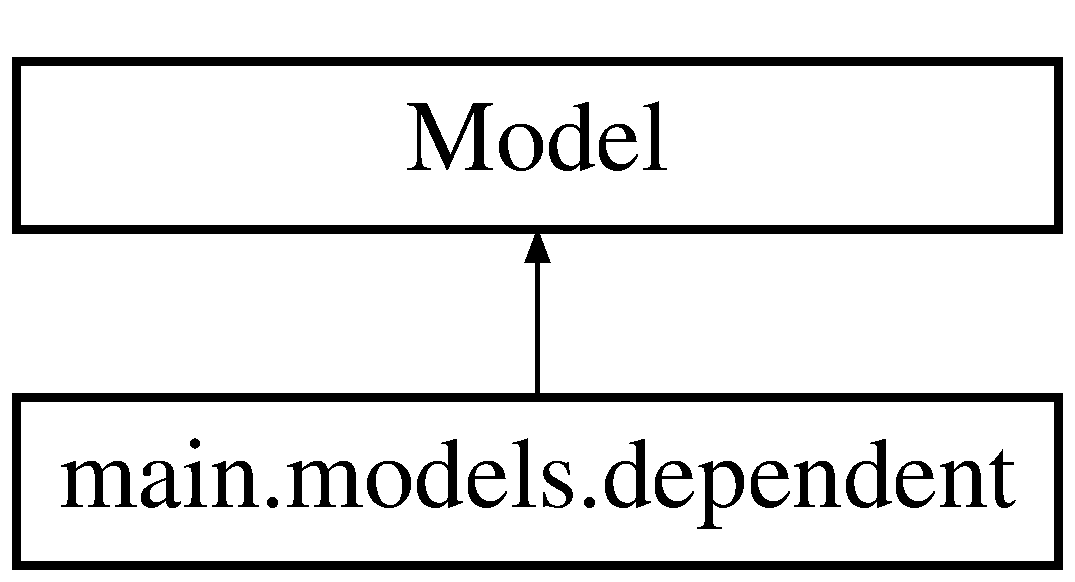
\includegraphics[height=2.000000cm]{classmain_1_1models_1_1dependent}
\end{center}
\end{figure}
\subsection*{Public Member Functions}
\begin{DoxyCompactItemize}
\item 
def \hyperlink{classmain_1_1models_1_1dependent_a03bbd4008311076414605382595dd174}{\+\_\+\+\_\+str\+\_\+\+\_\+} (self)
\end{DoxyCompactItemize}
\subsection*{Static Public Attributes}
\begin{DoxyCompactItemize}
\item 
\hyperlink{classmain_1_1models_1_1dependent_a73f6cd97e7cabd931b7d543ac1fb04ba}{staff\+\_\+name} = models.\+Char\+Field(max\+\_\+length=200, default=\char`\"{}D\+U\+M\+MY\char`\"{})
\begin{DoxyCompactList}\small\item\em Username of the staff. \end{DoxyCompactList}\item 
\hyperlink{classmain_1_1models_1_1dependent_a2a9f10a83b2253ec10314e4d044f00c0}{supervisor\+\_\+name} = models.\+Char\+Field(max\+\_\+length=200)
\begin{DoxyCompactList}\small\item\em Username of the supervisor. \end{DoxyCompactList}\end{DoxyCompactItemize}


\subsection{Detailed Description}
Defines the model to store all the staff-\/supervisor mappings. 

\subsection{Member Function Documentation}
\mbox{\Hypertarget{classmain_1_1models_1_1dependent_a03bbd4008311076414605382595dd174}\label{classmain_1_1models_1_1dependent_a03bbd4008311076414605382595dd174}} 
\index{main\+::models\+::dependent@{main\+::models\+::dependent}!\+\_\+\+\_\+str\+\_\+\+\_\+@{\+\_\+\+\_\+str\+\_\+\+\_\+}}
\index{\+\_\+\+\_\+str\+\_\+\+\_\+@{\+\_\+\+\_\+str\+\_\+\+\_\+}!main\+::models\+::dependent@{main\+::models\+::dependent}}
\subsubsection{\texorpdfstring{\+\_\+\+\_\+str\+\_\+\+\_\+()}{\_\_str\_\_()}}
{\footnotesize\ttfamily def main.\+models.\+dependent.\+\_\+\+\_\+str\+\_\+\+\_\+ (\begin{DoxyParamCaption}\item[{}]{self }\end{DoxyParamCaption})}



\subsection{Member Data Documentation}
\mbox{\Hypertarget{classmain_1_1models_1_1dependent_a73f6cd97e7cabd931b7d543ac1fb04ba}\label{classmain_1_1models_1_1dependent_a73f6cd97e7cabd931b7d543ac1fb04ba}} 
\index{main\+::models\+::dependent@{main\+::models\+::dependent}!staff\+\_\+name@{staff\+\_\+name}}
\index{staff\+\_\+name@{staff\+\_\+name}!main\+::models\+::dependent@{main\+::models\+::dependent}}
\subsubsection{\texorpdfstring{staff\+\_\+name}{staff\_name}}
{\footnotesize\ttfamily main.\+models.\+dependent.\+staff\+\_\+name = models.\+Char\+Field(max\+\_\+length=200, default=\char`\"{}D\+U\+M\+MY\char`\"{})\hspace{0.3cm}{\ttfamily [static]}}



Username of the staff. 

\mbox{\Hypertarget{classmain_1_1models_1_1dependent_a2a9f10a83b2253ec10314e4d044f00c0}\label{classmain_1_1models_1_1dependent_a2a9f10a83b2253ec10314e4d044f00c0}} 
\index{main\+::models\+::dependent@{main\+::models\+::dependent}!supervisor\+\_\+name@{supervisor\+\_\+name}}
\index{supervisor\+\_\+name@{supervisor\+\_\+name}!main\+::models\+::dependent@{main\+::models\+::dependent}}
\subsubsection{\texorpdfstring{supervisor\+\_\+name}{supervisor\_name}}
{\footnotesize\ttfamily main.\+models.\+dependent.\+supervisor\+\_\+name = models.\+Char\+Field(max\+\_\+length=200)\hspace{0.3cm}{\ttfamily [static]}}



Username of the supervisor. 



The documentation for this class was generated from the following file\+:\begin{DoxyCompactItemize}
\item 
main/\hyperlink{models_8py}{models.\+py}\end{DoxyCompactItemize}

\hypertarget{classmain_1_1models_1_1Leave}{}\section{main.\+models.\+Leave Class Reference}
\label{classmain_1_1models_1_1Leave}\index{main.\+models.\+Leave@{main.\+models.\+Leave}}


Defines the model to store all the leave\+\_\+requests-\/related details.  


Inheritance diagram for main.\+models.\+Leave\+:\begin{figure}[H]
\begin{center}
\leavevmode
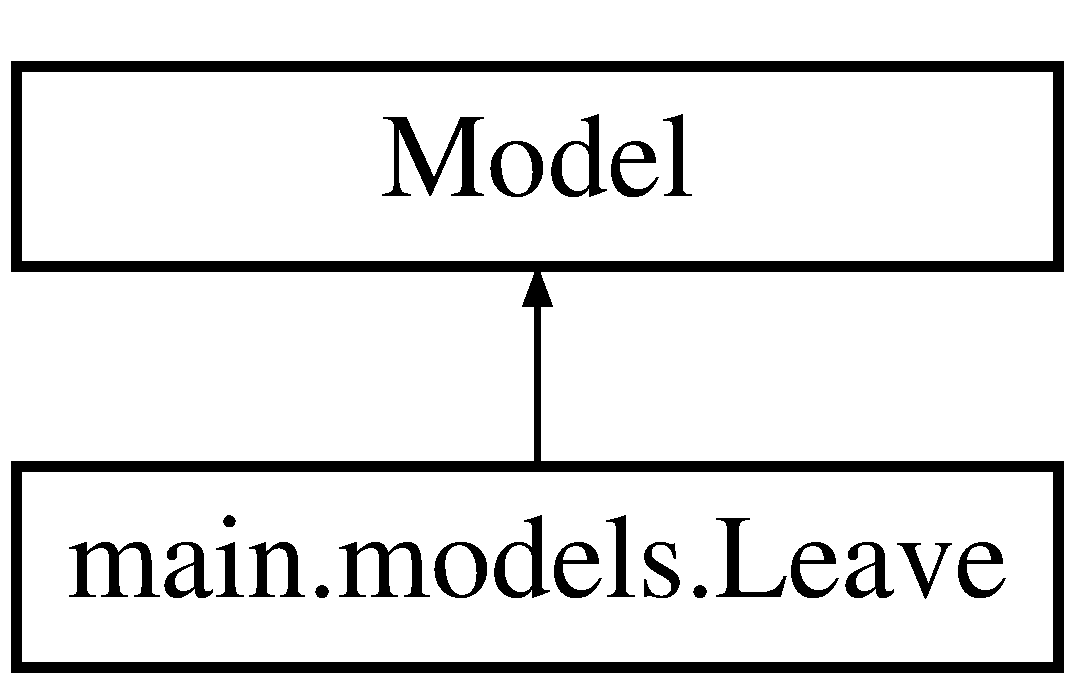
\includegraphics[height=2.000000cm]{classmain_1_1models_1_1Leave}
\end{center}
\end{figure}
\subsection*{Public Member Functions}
\begin{DoxyCompactItemize}
\item 
def \hyperlink{classmain_1_1models_1_1Leave_a79313821dfa94be8abab7a134808b972}{\+\_\+\+\_\+str\+\_\+\+\_\+} (self)
\end{DoxyCompactItemize}
\subsection*{Static Public Attributes}
\begin{DoxyCompactItemize}
\item 
\hyperlink{classmain_1_1models_1_1Leave_ad385bab40efa61e41021f8bdeccfbd4f}{start\+\_\+date} = models.\+Date\+Field(\char`\"{}start date\char`\"{})
\begin{DoxyCompactList}\small\item\em Start date of the leave period. \end{DoxyCompactList}\item 
\hyperlink{classmain_1_1models_1_1Leave_a99445fa4624f6668e3e881e0612ebd10}{no\+\_\+of\+\_\+days} = models.\+Integer\+Field()
\begin{DoxyCompactList}\small\item\em Total no of days in the leave period. \end{DoxyCompactList}\item 
\hyperlink{classmain_1_1models_1_1Leave_af65436e87a630c5d204bb91f8c0ccf01}{reason} = models.\+Text\+Field()
\begin{DoxyCompactList}\small\item\em Reason for the leave request. \end{DoxyCompactList}\item 
\hyperlink{classmain_1_1models_1_1Leave_a5a7ee37588c877c656b587b091051bf4}{approved} = models.\+Boolean\+Field(default=\textquotesingle{}false\textquotesingle{})
\begin{DoxyCompactList}\small\item\em Approval status of the request. \end{DoxyCompactList}\item 
\hyperlink{classmain_1_1models_1_1Leave_a062e4dd38d8e161c3b50a0b6cf7095f2}{author} = models.\+Char\+Field(max\+\_\+length=200,default=\char`\"{}Author\char`\"{})
\begin{DoxyCompactList}\small\item\em username of the staff who applied for the leave \end{DoxyCompactList}\end{DoxyCompactItemize}


\subsection{Detailed Description}
Defines the model to store all the leave\+\_\+requests-\/related details. 

\subsection{Member Function Documentation}
\mbox{\Hypertarget{classmain_1_1models_1_1Leave_a79313821dfa94be8abab7a134808b972}\label{classmain_1_1models_1_1Leave_a79313821dfa94be8abab7a134808b972}} 
\index{main\+::models\+::\+Leave@{main\+::models\+::\+Leave}!\+\_\+\+\_\+str\+\_\+\+\_\+@{\+\_\+\+\_\+str\+\_\+\+\_\+}}
\index{\+\_\+\+\_\+str\+\_\+\+\_\+@{\+\_\+\+\_\+str\+\_\+\+\_\+}!main\+::models\+::\+Leave@{main\+::models\+::\+Leave}}
\subsubsection{\texorpdfstring{\+\_\+\+\_\+str\+\_\+\+\_\+()}{\_\_str\_\_()}}
{\footnotesize\ttfamily def main.\+models.\+Leave.\+\_\+\+\_\+str\+\_\+\+\_\+ (\begin{DoxyParamCaption}\item[{}]{self }\end{DoxyParamCaption})}



\subsection{Member Data Documentation}
\mbox{\Hypertarget{classmain_1_1models_1_1Leave_a5a7ee37588c877c656b587b091051bf4}\label{classmain_1_1models_1_1Leave_a5a7ee37588c877c656b587b091051bf4}} 
\index{main\+::models\+::\+Leave@{main\+::models\+::\+Leave}!approved@{approved}}
\index{approved@{approved}!main\+::models\+::\+Leave@{main\+::models\+::\+Leave}}
\subsubsection{\texorpdfstring{approved}{approved}}
{\footnotesize\ttfamily main.\+models.\+Leave.\+approved = models.\+Boolean\+Field(default=\textquotesingle{}false\textquotesingle{})\hspace{0.3cm}{\ttfamily [static]}}



Approval status of the request. 

\mbox{\Hypertarget{classmain_1_1models_1_1Leave_a062e4dd38d8e161c3b50a0b6cf7095f2}\label{classmain_1_1models_1_1Leave_a062e4dd38d8e161c3b50a0b6cf7095f2}} 
\index{main\+::models\+::\+Leave@{main\+::models\+::\+Leave}!author@{author}}
\index{author@{author}!main\+::models\+::\+Leave@{main\+::models\+::\+Leave}}
\subsubsection{\texorpdfstring{author}{author}}
{\footnotesize\ttfamily main.\+models.\+Leave.\+author = models.\+Char\+Field(max\+\_\+length=200,default=\char`\"{}Author\char`\"{})\hspace{0.3cm}{\ttfamily [static]}}



username of the staff who applied for the leave 

\mbox{\Hypertarget{classmain_1_1models_1_1Leave_a99445fa4624f6668e3e881e0612ebd10}\label{classmain_1_1models_1_1Leave_a99445fa4624f6668e3e881e0612ebd10}} 
\index{main\+::models\+::\+Leave@{main\+::models\+::\+Leave}!no\+\_\+of\+\_\+days@{no\+\_\+of\+\_\+days}}
\index{no\+\_\+of\+\_\+days@{no\+\_\+of\+\_\+days}!main\+::models\+::\+Leave@{main\+::models\+::\+Leave}}
\subsubsection{\texorpdfstring{no\+\_\+of\+\_\+days}{no\_of\_days}}
{\footnotesize\ttfamily main.\+models.\+Leave.\+no\+\_\+of\+\_\+days = models.\+Integer\+Field()\hspace{0.3cm}{\ttfamily [static]}}



Total no of days in the leave period. 

\mbox{\Hypertarget{classmain_1_1models_1_1Leave_af65436e87a630c5d204bb91f8c0ccf01}\label{classmain_1_1models_1_1Leave_af65436e87a630c5d204bb91f8c0ccf01}} 
\index{main\+::models\+::\+Leave@{main\+::models\+::\+Leave}!reason@{reason}}
\index{reason@{reason}!main\+::models\+::\+Leave@{main\+::models\+::\+Leave}}
\subsubsection{\texorpdfstring{reason}{reason}}
{\footnotesize\ttfamily main.\+models.\+Leave.\+reason = models.\+Text\+Field()\hspace{0.3cm}{\ttfamily [static]}}



Reason for the leave request. 

\mbox{\Hypertarget{classmain_1_1models_1_1Leave_ad385bab40efa61e41021f8bdeccfbd4f}\label{classmain_1_1models_1_1Leave_ad385bab40efa61e41021f8bdeccfbd4f}} 
\index{main\+::models\+::\+Leave@{main\+::models\+::\+Leave}!start\+\_\+date@{start\+\_\+date}}
\index{start\+\_\+date@{start\+\_\+date}!main\+::models\+::\+Leave@{main\+::models\+::\+Leave}}
\subsubsection{\texorpdfstring{start\+\_\+date}{start\_date}}
{\footnotesize\ttfamily main.\+models.\+Leave.\+start\+\_\+date = models.\+Date\+Field(\char`\"{}start date\char`\"{})\hspace{0.3cm}{\ttfamily [static]}}



Start date of the leave period. 



The documentation for this class was generated from the following file\+:\begin{DoxyCompactItemize}
\item 
main/\hyperlink{models_8py}{models.\+py}\end{DoxyCompactItemize}

\hypertarget{classmain_1_1forms_1_1LeaveForm}{}\section{main.\+forms.\+Leave\+Form Class Reference}
\label{classmain_1_1forms_1_1LeaveForm}\index{main.\+forms.\+Leave\+Form@{main.\+forms.\+Leave\+Form}}


Creates a form for the Leave model, using the django Model\+Form.  


Inheritance diagram for main.\+forms.\+Leave\+Form\+:\begin{figure}[H]
\begin{center}
\leavevmode
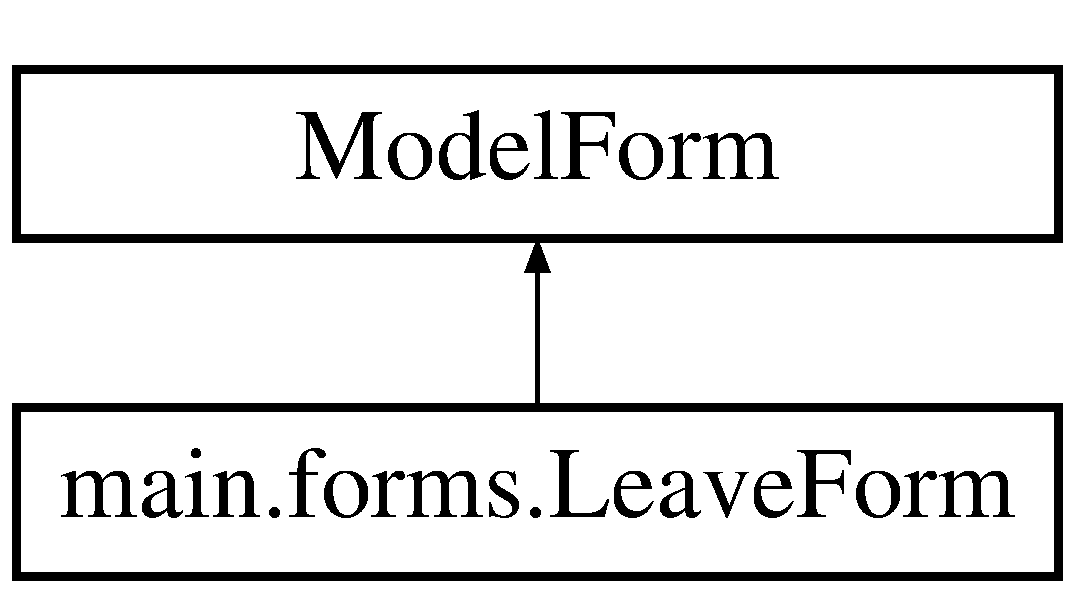
\includegraphics[height=2.000000cm]{classmain_1_1forms_1_1LeaveForm}
\end{center}
\end{figure}


\subsection{Detailed Description}
Creates a form for the Leave model, using the django Model\+Form. 

Used to take input the leave request details posted by the staff and store them in the Leave model. The author and approved field is kept hidden. Class Meta\+: An inner class to provide metadata to the Model\+Form class. Provides an association between the Model\+Form and the model Leave. 

The documentation for this class was generated from the following file\+:\begin{DoxyCompactItemize}
\item 
main/\hyperlink{forms_8py}{forms.\+py}\end{DoxyCompactItemize}

\hypertarget{classmain_1_1apps_1_1MainConfig}{}\section{main.\+apps.\+Main\+Config Class Reference}
\label{classmain_1_1apps_1_1MainConfig}\index{main.\+apps.\+Main\+Config@{main.\+apps.\+Main\+Config}}
Inheritance diagram for main.\+apps.\+Main\+Config\+:\begin{figure}[H]
\begin{center}
\leavevmode
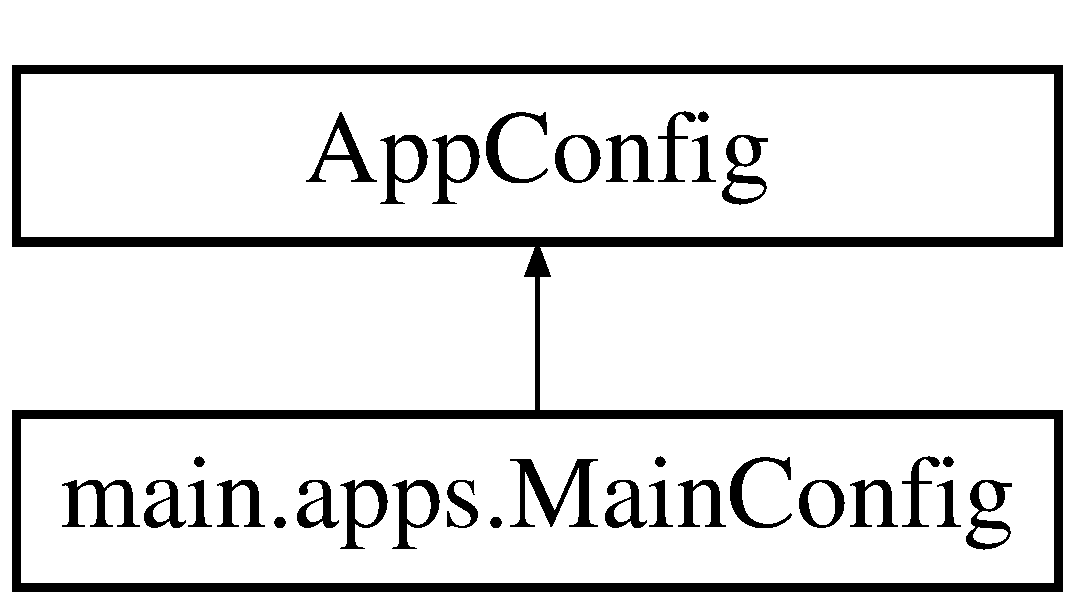
\includegraphics[height=2.000000cm]{classmain_1_1apps_1_1MainConfig}
\end{center}
\end{figure}
\subsection*{Static Public Attributes}
\begin{DoxyCompactItemize}
\item 
string \hyperlink{classmain_1_1apps_1_1MainConfig_aa4f22f649b0536d455304a3d137d6b2c}{name} = \textquotesingle{}main\textquotesingle{}
\end{DoxyCompactItemize}


\subsection{Member Data Documentation}
\mbox{\Hypertarget{classmain_1_1apps_1_1MainConfig_aa4f22f649b0536d455304a3d137d6b2c}\label{classmain_1_1apps_1_1MainConfig_aa4f22f649b0536d455304a3d137d6b2c}} 
\index{main\+::apps\+::\+Main\+Config@{main\+::apps\+::\+Main\+Config}!name@{name}}
\index{name@{name}!main\+::apps\+::\+Main\+Config@{main\+::apps\+::\+Main\+Config}}
\subsubsection{\texorpdfstring{name}{name}}
{\footnotesize\ttfamily string main.\+apps.\+Main\+Config.\+name = \textquotesingle{}main\textquotesingle{}\hspace{0.3cm}{\ttfamily [static]}}



The documentation for this class was generated from the following file\+:\begin{DoxyCompactItemize}
\item 
main/\hyperlink{apps_8py}{apps.\+py}\end{DoxyCompactItemize}

\hypertarget{classmain_1_1models_1_1Posts}{}\section{main.\+models.\+Posts Class Reference}
\label{classmain_1_1models_1_1Posts}\index{main.\+models.\+Posts@{main.\+models.\+Posts}}


Defines the model to store all the post-\/related details.  


Inheritance diagram for main.\+models.\+Posts\+:\begin{figure}[H]
\begin{center}
\leavevmode
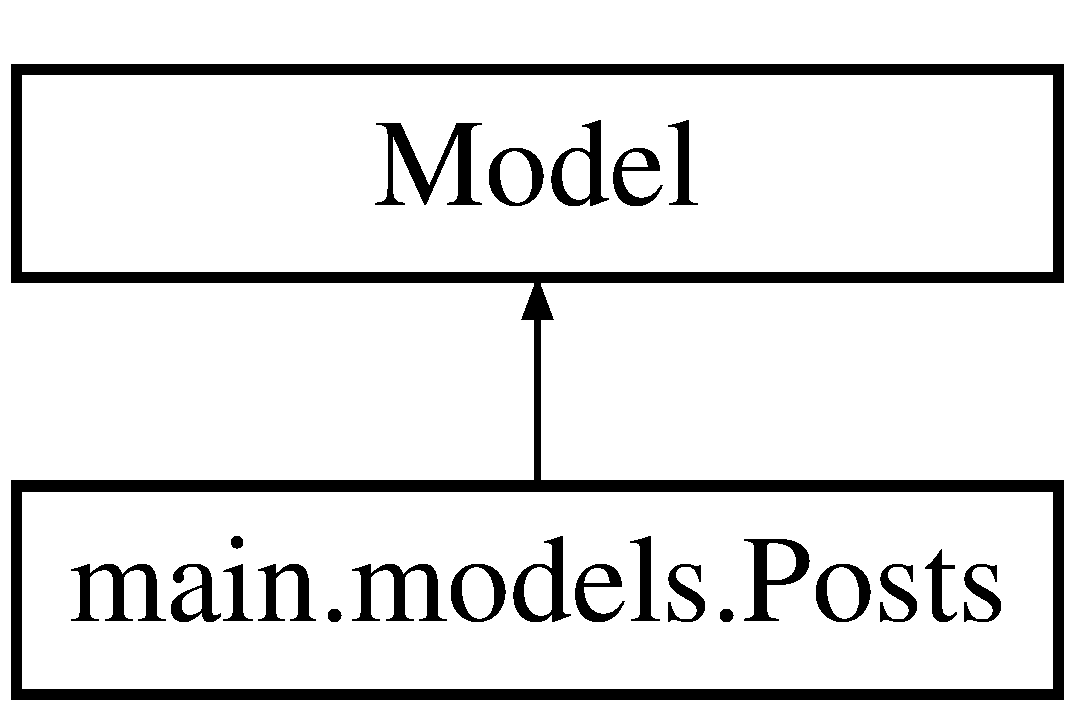
\includegraphics[height=2.000000cm]{classmain_1_1models_1_1Posts}
\end{center}
\end{figure}
\subsection*{Public Member Functions}
\begin{DoxyCompactItemize}
\item 
def \hyperlink{classmain_1_1models_1_1Posts_a1beebe8f01eb6f1cf42f33a877c1b73a}{\+\_\+\+\_\+str\+\_\+\+\_\+} (self)
\end{DoxyCompactItemize}
\subsection*{Static Public Attributes}
\begin{DoxyCompactItemize}
\item 
\hyperlink{classmain_1_1models_1_1Posts_aff937f03c1b067fa1dbc22fe0a4f141c}{job\+\_\+title} = models.\+Char\+Field(max\+\_\+length=200)
\begin{DoxyCompactList}\small\item\em The title of the post. \end{DoxyCompactList}\item 
\hyperlink{classmain_1_1models_1_1Posts_a6a7cef4a2cff2cb38557a346b1b9cc9e}{job\+\_\+location} = models.\+Char\+Field(max\+\_\+length=100,default=\char`\"{}Hostel\+X\+YZ\char`\"{})
\begin{DoxyCompactList}\small\item\em Location of the job. \end{DoxyCompactList}\item 
\hyperlink{classmain_1_1models_1_1Posts_a8d5fd2451a74cbef923c841192627ee4}{job\+\_\+date} = models.\+Date\+Time\+Field(\char`\"{}job date\char`\"{},default=datetime.\+now())
\begin{DoxyCompactList}\small\item\em date of job \end{DoxyCompactList}\item 
\hyperlink{classmain_1_1models_1_1Posts_a01fb86493104e3ed82c25b011b4768a7}{job\+\_\+details} = models.\+Text\+Field()
\begin{DoxyCompactList}\small\item\em A brief description of the job. \end{DoxyCompactList}\item 
\hyperlink{classmain_1_1models_1_1Posts_a6e0e50f0ed5e44dc5b275de570745348}{post\+\_\+published} = models.\+Date\+Time\+Field(\char`\"{}date published\char`\"{},default=datetime.\+now())
\begin{DoxyCompactList}\small\item\em Date when the post was published. \end{DoxyCompactList}\item 
\hyperlink{classmain_1_1models_1_1Posts_ab030c90138407de66474824c18a2ef28}{author} = models.\+Char\+Field(max\+\_\+length=200,default=\char`\"{}Author\char`\"{})
\begin{DoxyCompactList}\small\item\em username of the person who created the post \end{DoxyCompactList}\end{DoxyCompactItemize}


\subsection{Detailed Description}
Defines the model to store all the post-\/related details. 

\subsection{Member Function Documentation}
\mbox{\Hypertarget{classmain_1_1models_1_1Posts_a1beebe8f01eb6f1cf42f33a877c1b73a}\label{classmain_1_1models_1_1Posts_a1beebe8f01eb6f1cf42f33a877c1b73a}} 
\index{main\+::models\+::\+Posts@{main\+::models\+::\+Posts}!\+\_\+\+\_\+str\+\_\+\+\_\+@{\+\_\+\+\_\+str\+\_\+\+\_\+}}
\index{\+\_\+\+\_\+str\+\_\+\+\_\+@{\+\_\+\+\_\+str\+\_\+\+\_\+}!main\+::models\+::\+Posts@{main\+::models\+::\+Posts}}
\subsubsection{\texorpdfstring{\+\_\+\+\_\+str\+\_\+\+\_\+()}{\_\_str\_\_()}}
{\footnotesize\ttfamily def main.\+models.\+Posts.\+\_\+\+\_\+str\+\_\+\+\_\+ (\begin{DoxyParamCaption}\item[{}]{self }\end{DoxyParamCaption})}



\subsection{Member Data Documentation}
\mbox{\Hypertarget{classmain_1_1models_1_1Posts_ab030c90138407de66474824c18a2ef28}\label{classmain_1_1models_1_1Posts_ab030c90138407de66474824c18a2ef28}} 
\index{main\+::models\+::\+Posts@{main\+::models\+::\+Posts}!author@{author}}
\index{author@{author}!main\+::models\+::\+Posts@{main\+::models\+::\+Posts}}
\subsubsection{\texorpdfstring{author}{author}}
{\footnotesize\ttfamily main.\+models.\+Posts.\+author = models.\+Char\+Field(max\+\_\+length=200,default=\char`\"{}Author\char`\"{})\hspace{0.3cm}{\ttfamily [static]}}



username of the person who created the post 

\mbox{\Hypertarget{classmain_1_1models_1_1Posts_a8d5fd2451a74cbef923c841192627ee4}\label{classmain_1_1models_1_1Posts_a8d5fd2451a74cbef923c841192627ee4}} 
\index{main\+::models\+::\+Posts@{main\+::models\+::\+Posts}!job\+\_\+date@{job\+\_\+date}}
\index{job\+\_\+date@{job\+\_\+date}!main\+::models\+::\+Posts@{main\+::models\+::\+Posts}}
\subsubsection{\texorpdfstring{job\+\_\+date}{job\_date}}
{\footnotesize\ttfamily main.\+models.\+Posts.\+job\+\_\+date = models.\+Date\+Time\+Field(\char`\"{}job date\char`\"{},default=datetime.\+now())\hspace{0.3cm}{\ttfamily [static]}}



date of job 

\mbox{\Hypertarget{classmain_1_1models_1_1Posts_a01fb86493104e3ed82c25b011b4768a7}\label{classmain_1_1models_1_1Posts_a01fb86493104e3ed82c25b011b4768a7}} 
\index{main\+::models\+::\+Posts@{main\+::models\+::\+Posts}!job\+\_\+details@{job\+\_\+details}}
\index{job\+\_\+details@{job\+\_\+details}!main\+::models\+::\+Posts@{main\+::models\+::\+Posts}}
\subsubsection{\texorpdfstring{job\+\_\+details}{job\_details}}
{\footnotesize\ttfamily main.\+models.\+Posts.\+job\+\_\+details = models.\+Text\+Field()\hspace{0.3cm}{\ttfamily [static]}}



A brief description of the job. 

\mbox{\Hypertarget{classmain_1_1models_1_1Posts_a6a7cef4a2cff2cb38557a346b1b9cc9e}\label{classmain_1_1models_1_1Posts_a6a7cef4a2cff2cb38557a346b1b9cc9e}} 
\index{main\+::models\+::\+Posts@{main\+::models\+::\+Posts}!job\+\_\+location@{job\+\_\+location}}
\index{job\+\_\+location@{job\+\_\+location}!main\+::models\+::\+Posts@{main\+::models\+::\+Posts}}
\subsubsection{\texorpdfstring{job\+\_\+location}{job\_location}}
{\footnotesize\ttfamily main.\+models.\+Posts.\+job\+\_\+location = models.\+Char\+Field(max\+\_\+length=100,default=\char`\"{}Hostel\+X\+YZ\char`\"{})\hspace{0.3cm}{\ttfamily [static]}}



Location of the job. 

\mbox{\Hypertarget{classmain_1_1models_1_1Posts_aff937f03c1b067fa1dbc22fe0a4f141c}\label{classmain_1_1models_1_1Posts_aff937f03c1b067fa1dbc22fe0a4f141c}} 
\index{main\+::models\+::\+Posts@{main\+::models\+::\+Posts}!job\+\_\+title@{job\+\_\+title}}
\index{job\+\_\+title@{job\+\_\+title}!main\+::models\+::\+Posts@{main\+::models\+::\+Posts}}
\subsubsection{\texorpdfstring{job\+\_\+title}{job\_title}}
{\footnotesize\ttfamily main.\+models.\+Posts.\+job\+\_\+title = models.\+Char\+Field(max\+\_\+length=200)\hspace{0.3cm}{\ttfamily [static]}}



The title of the post. 

\mbox{\Hypertarget{classmain_1_1models_1_1Posts_a6e0e50f0ed5e44dc5b275de570745348}\label{classmain_1_1models_1_1Posts_a6e0e50f0ed5e44dc5b275de570745348}} 
\index{main\+::models\+::\+Posts@{main\+::models\+::\+Posts}!post\+\_\+published@{post\+\_\+published}}
\index{post\+\_\+published@{post\+\_\+published}!main\+::models\+::\+Posts@{main\+::models\+::\+Posts}}
\subsubsection{\texorpdfstring{post\+\_\+published}{post\_published}}
{\footnotesize\ttfamily main.\+models.\+Posts.\+post\+\_\+published = models.\+Date\+Time\+Field(\char`\"{}date published\char`\"{},default=datetime.\+now())\hspace{0.3cm}{\ttfamily [static]}}



Date when the post was published. 



The documentation for this class was generated from the following file\+:\begin{DoxyCompactItemize}
\item 
main/\hyperlink{models_8py}{models.\+py}\end{DoxyCompactItemize}

\hypertarget{classmain_1_1forms_1_1PostsForm}{}\section{main.\+forms.\+Posts\+Form Class Reference}
\label{classmain_1_1forms_1_1PostsForm}\index{main.\+forms.\+Posts\+Form@{main.\+forms.\+Posts\+Form}}


Creates a form for the Posts model, using the django Model\+Form.  


Inheritance diagram for main.\+forms.\+Posts\+Form\+:\begin{figure}[H]
\begin{center}
\leavevmode
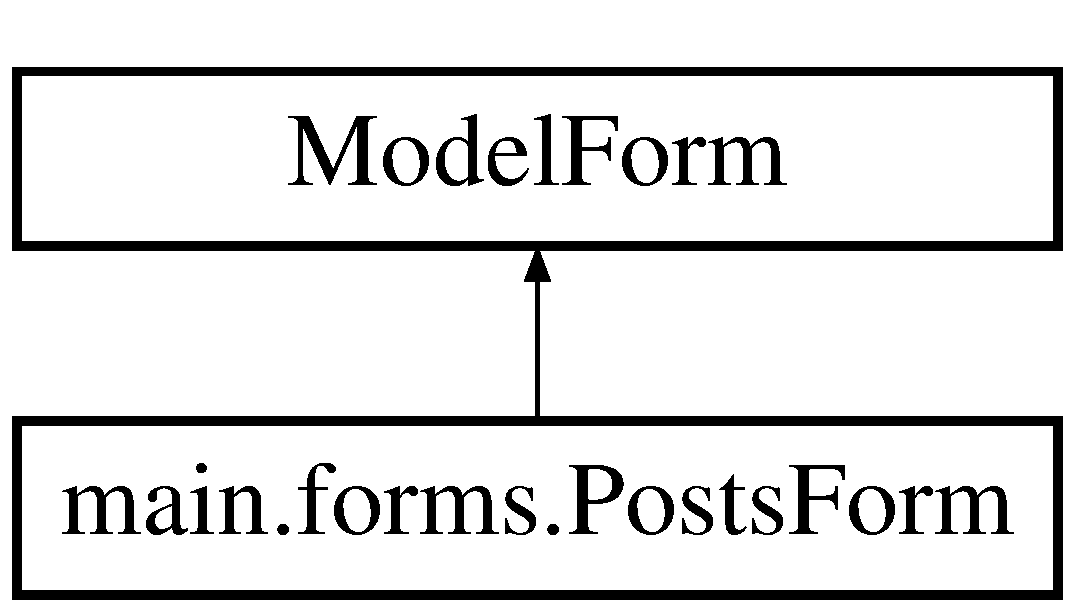
\includegraphics[height=2.000000cm]{classmain_1_1forms_1_1PostsForm}
\end{center}
\end{figure}


\subsection{Detailed Description}
Creates a form for the Posts model, using the django Model\+Form. 

Used to take input the job post details posted by the supervisor and store them in the Post model. The author and post\+\_\+published field is kept hidden. class Meta \+: An inner class to provide metadata to the Model\+Form class. Provides an association between the Model\+Form and the model Posts 

The documentation for this class was generated from the following file\+:\begin{DoxyCompactItemize}
\item 
main/\hyperlink{forms_8py}{forms.\+py}\end{DoxyCompactItemize}

\hypertarget{classmain_1_1forms_1_1selectForm}{}\section{main.\+forms.\+select\+Form Class Reference}
\label{classmain_1_1forms_1_1selectForm}\index{main.\+forms.\+select\+Form@{main.\+forms.\+select\+Form}}


Creates a form for the dependent model, using the django Model\+Form.  


Inheritance diagram for main.\+forms.\+select\+Form\+:\begin{figure}[H]
\begin{center}
\leavevmode
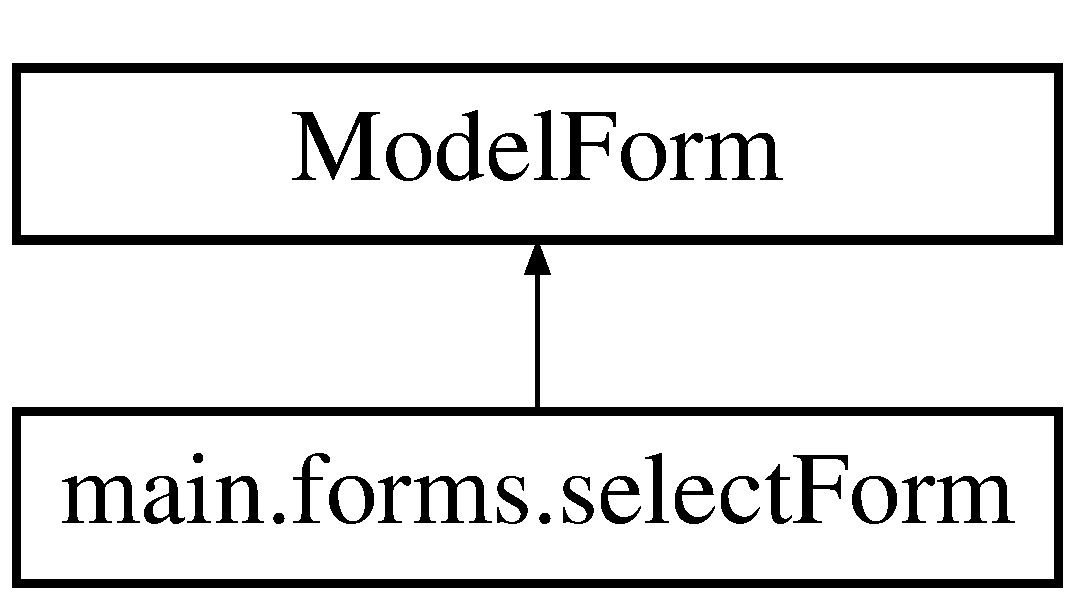
\includegraphics[height=2.000000cm]{classmain_1_1forms_1_1selectForm}
\end{center}
\end{figure}


\subsection{Detailed Description}
Creates a form for the dependent model, using the django Model\+Form. 

Used to take the supervisor of a current staff as input and store the supervisor-\/staff mapping in the dependent model. The staff\+\_\+name field is kept hidden. class Meta \+: An inner class to provide metadata to the Model\+Form class. Provides an association between the Model\+Form and the model dependent 

The documentation for this class was generated from the following file\+:\begin{DoxyCompactItemize}
\item 
main/\hyperlink{forms_8py}{forms.\+py}\end{DoxyCompactItemize}

\chapter{File Documentation}
\hypertarget{____init_____8py}{}\section{main/\+\_\+\+\_\+init\+\_\+\+\_\+.py File Reference}
\label{____init_____8py}\index{main/\+\_\+\+\_\+init\+\_\+\+\_\+.\+py@{main/\+\_\+\+\_\+init\+\_\+\+\_\+.\+py}}
\subsection*{Namespaces}
\begin{DoxyCompactItemize}
\item 
 \hyperlink{namespacemain}{main}
\end{DoxyCompactItemize}

\hypertarget{admin_8py}{}\section{main/admin.py File Reference}
\label{admin_8py}\index{main/admin.\+py@{main/admin.\+py}}
\subsection*{Namespaces}
\begin{DoxyCompactItemize}
\item 
 \hyperlink{namespacemain_1_1admin}{main.\+admin}
\end{DoxyCompactItemize}

\hypertarget{apps_8py}{}\section{main/apps.py File Reference}
\label{apps_8py}\index{main/apps.\+py@{main/apps.\+py}}
\subsection*{Classes}
\begin{DoxyCompactItemize}
\item 
class \hyperlink{classmain_1_1apps_1_1MainConfig}{main.\+apps.\+Main\+Config}
\end{DoxyCompactItemize}
\subsection*{Namespaces}
\begin{DoxyCompactItemize}
\item 
 \hyperlink{namespacemain_1_1apps}{main.\+apps}
\end{DoxyCompactItemize}

\hypertarget{forms_8py}{}\section{main/forms.py File Reference}
\label{forms_8py}\index{main/forms.\+py@{main/forms.\+py}}
\subsection*{Classes}
\begin{DoxyCompactItemize}
\item 
class \hyperlink{classmain_1_1forms_1_1selectForm}{main.\+forms.\+select\+Form}
\begin{DoxyCompactList}\small\item\em Creates a form for the dependent model, using the django Model\+Form. \end{DoxyCompactList}\item 
class \hyperlink{classmain_1_1forms_1_1PostsForm}{main.\+forms.\+Posts\+Form}
\begin{DoxyCompactList}\small\item\em Creates a form for the Posts model, using the django Model\+Form. \end{DoxyCompactList}\item 
class \hyperlink{classmain_1_1forms_1_1LeaveForm}{main.\+forms.\+Leave\+Form}
\begin{DoxyCompactList}\small\item\em Creates a form for the Leave model, using the django Model\+Form. \end{DoxyCompactList}\end{DoxyCompactItemize}
\subsection*{Namespaces}
\begin{DoxyCompactItemize}
\item 
 \hyperlink{namespacemain_1_1forms}{main.\+forms}
\end{DoxyCompactItemize}

\hypertarget{models_8py}{}\section{main/models.py File Reference}
\label{models_8py}\index{main/models.\+py@{main/models.\+py}}
\subsection*{Classes}
\begin{DoxyCompactItemize}
\item 
class \hyperlink{classmain_1_1models_1_1Posts}{main.\+models.\+Posts}
\begin{DoxyCompactList}\small\item\em Defines the model to store all the post-\/related details. \end{DoxyCompactList}\item 
class \hyperlink{classmain_1_1models_1_1Leave}{main.\+models.\+Leave}
\begin{DoxyCompactList}\small\item\em Defines the model to store all the leave\+\_\+requests-\/related details. \end{DoxyCompactList}\item 
class \hyperlink{classmain_1_1models_1_1dependent}{main.\+models.\+dependent}
\begin{DoxyCompactList}\small\item\em Defines the model to store all the staff-\/supervisor mappings. \end{DoxyCompactList}\end{DoxyCompactItemize}
\subsection*{Namespaces}
\begin{DoxyCompactItemize}
\item 
 \hyperlink{namespacemain_1_1models}{main.\+models}
\end{DoxyCompactItemize}

\hypertarget{tests_8py}{}\section{main/tests.py File Reference}
\label{tests_8py}\index{main/tests.\+py@{main/tests.\+py}}
\subsection*{Namespaces}
\begin{DoxyCompactItemize}
\item 
 \hyperlink{namespacemain_1_1tests}{main.\+tests}
\end{DoxyCompactItemize}

\hypertarget{urls_8py}{}\section{main/urls.py File Reference}
\label{urls_8py}\index{main/urls.\+py@{main/urls.\+py}}
\subsection*{Namespaces}
\begin{DoxyCompactItemize}
\item 
 \hyperlink{namespacemain_1_1urls}{main.\+urls}
\end{DoxyCompactItemize}
\subsection*{Variables}
\begin{DoxyCompactItemize}
\item 
string \hyperlink{namespacemain_1_1urls_a51dcca3e024577b219fd64d918455026}{main.\+urls.\+app\+\_\+name} = \char`\"{}main\char`\"{}
\item 
list \hyperlink{namespacemain_1_1urls_a49ff062cbecb056ec955c38ee8b784c3}{main.\+urls.\+urlpatterns}
\begin{DoxyCompactList}\small\item\em contain the url patterns and their respective views \end{DoxyCompactList}\end{DoxyCompactItemize}

\hypertarget{views_8py}{}\section{main/views.py File Reference}
\label{views_8py}\index{main/views.\+py@{main/views.\+py}}
\subsection*{Namespaces}
\begin{DoxyCompactItemize}
\item 
 \hyperlink{namespacemain_1_1views}{main.\+views}
\end{DoxyCompactItemize}
\subsection*{Functions}
\begin{DoxyCompactItemize}
\item 
def \hyperlink{namespacemain_1_1views_a65a9dba6e3878ee1da013593b60345d4}{main.\+views.\+homepage} (request)
\begin{DoxyCompactList}\small\item\em Defines what action to perform when the view \textquotesingle{}homepage\textquotesingle{} is called from urls. \end{DoxyCompactList}\item 
def \hyperlink{namespacemain_1_1views_a33ddb0f904d196b5830dbb9a1a8f1282}{main.\+views.\+posts} (request)
\begin{DoxyCompactList}\small\item\em Defines what action to perform when the view \textquotesingle{}posts\textquotesingle{} is called from urls. \end{DoxyCompactList}\item 
def \hyperlink{namespacemain_1_1views_acdd49ab16815f9d6cb3e88feab0bfa80}{main.\+views.\+leave\+\_\+requests} (request)
\begin{DoxyCompactList}\small\item\em Defines what action to perform when the view \textquotesingle{}leave\+\_\+requests\textquotesingle{} is called from urls. \end{DoxyCompactList}\item 
def \hyperlink{namespacemain_1_1views_abdf62da100e2d6945871318f111c478c}{main.\+views.\+select\+\_\+supervisor} (request)
\begin{DoxyCompactList}\small\item\em Defines what action to perform when the view \textquotesingle{}select\+\_\+supervisor\textquotesingle{} is called from urls. \end{DoxyCompactList}\item 
def \hyperlink{namespacemain_1_1views_a5188f01b8c7ed850b1f946afb34d183a}{main.\+views.\+create\+\_\+posts} (request)
\begin{DoxyCompactList}\small\item\em Defines what action to perform when the view \textquotesingle{}create\+\_\+posts\textquotesingle{} is called from urls. \end{DoxyCompactList}\item 
def \hyperlink{namespacemain_1_1views_a0e05992f5c64ffb3cd35ddc581399e31}{main.\+views.\+leave} (request)
\begin{DoxyCompactList}\small\item\em Defines what action to perform when the view \textquotesingle{}leave\textquotesingle{} is called from urls. \end{DoxyCompactList}\item 
def \hyperlink{namespacemain_1_1views_a36b45d6ab9335da129aeab31c613726a}{main.\+views.\+register} (request)
\begin{DoxyCompactList}\small\item\em Defines what action to perform when the view \textquotesingle{}register\textquotesingle{} is called from urls. \end{DoxyCompactList}\item 
def \hyperlink{namespacemain_1_1views_afa83b35a6a0c354a6d9878bc3584aae4}{main.\+views.\+register\+\_\+staff} (request)
\begin{DoxyCompactList}\small\item\em Defines what action to perform when the view \textquotesingle{}register\+\_\+staff\textquotesingle{} is called from urls. \end{DoxyCompactList}\item 
def \hyperlink{namespacemain_1_1views_a26d1574cf1c0681b1589baf8f2840e4a}{main.\+views.\+register\+\_\+supervisor} (request)
\begin{DoxyCompactList}\small\item\em Defines what action to perform when the view \textquotesingle{}register\+\_\+supervisor\textquotesingle{} is called from urls. \end{DoxyCompactList}\item 
def \hyperlink{namespacemain_1_1views_a19ef1e1ff8dc4a8b7f24c011a69c56f5}{main.\+views.\+logout\+\_\+request} (request)
\begin{DoxyCompactList}\small\item\em Defines what action to perform when the view \textquotesingle{}logout\+\_\+request\textquotesingle{} is called from urls. \end{DoxyCompactList}\item 
def \hyperlink{namespacemain_1_1views_aa4b0b085bb5782a107fce5e03228e97b}{main.\+views.\+login\+\_\+request} (request)
\begin{DoxyCompactList}\small\item\em Defines what action to perform when the view \textquotesingle{}login\+\_\+request\textquotesingle{} is called from urls. \end{DoxyCompactList}\end{DoxyCompactItemize}

%--- End generated contents ---

% Index
\backmatter
\newpage
\phantomsection
\clearemptydoublepage
\addcontentsline{toc}{chapter}{Index}
\printindex

\end{document}
